\pdfoutput=1
\documentclass[11pt,a4paper]{article}
\usepackage[T1]{fontenc}
\usepackage[utf8]{inputenc}
\usepackage{amsmath,amssymb,amsthm}
\usepackage{mathtools}
\usepackage{mathrsfs}
\usepackage{slashed}
\usepackage{etoolbox}
\usepackage{graphicx}
\usepackage{tikz}
\usetikzlibrary{arrows.meta,calc,decorations.markings,decorations.pathmorphing}
\usepackage{jheppub}
\usepackage{pct}

\begin{document}
% PCT-SOURCE: pdf=023 print=011 kind=figure id=1-1
% Native reconstruction from the rendered source page.  The dashed outlines
% show the subgroup connectivity regions and the solid circles show the four
% components of the Lorentz group.
\begingroup
\renewcommand{\thefigure}{1-1}
\renewcommand{\figurename}{FIGURE}
\begin{figure}[t]
  \centering
  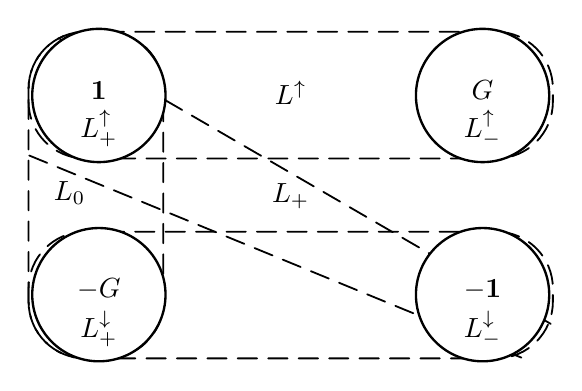
\begin{tikzpicture}[x=0.93cm,y=0.93cm,>=Stealth,
    line cap=round,line join=round]
    % The two horizontal subgroup regions.
    \draw[dashed,dash pattern=on 7pt off 4pt,line width=.65pt,
      rounded corners=0.72cm]
      (-3.58,0.50) rectangle (3.58,2.23);
    \draw[dashed,dash pattern=on 7pt off 4pt,line width=.65pt,
      rounded corners=0.72cm]
      (-3.58,-2.23) rectangle (3.58,-0.50);

    % The orthochorous subgroup and the proper subgroup are drawn behind the
    % component circles, as in the printed diagram.
    \draw[dashed,dash pattern=on 7pt off 4pt,line width=.65pt,
      rounded corners=0.72cm]
      (-3.58,-2.23) rectangle (-1.74,2.23);
    \draw[dashed,dash pattern=on 7pt off 4pt,line width=.65pt]
      (-3.15,2.13) -- (3.57,-1.77);
    \draw[dashed,dash pattern=on 7pt off 4pt,line width=.65pt]
      (-3.57,0.54) -- (3.15,-2.22);

    % The four connected components.
    \filldraw[fill=white,line width=.85pt] (-2.62,1.36) circle (0.91);
    \filldraw[fill=white,line width=.85pt] ( 2.62,1.36) circle (0.91);
    \filldraw[fill=white,line width=.85pt] (-2.62,-1.36) circle (0.91);
    \filldraw[fill=white,line width=.85pt] ( 2.62,-1.36) circle (0.91);

    \node at (-2.62,1.43) {$\mathbf{1}$};
    \node at ( 2.62,1.43) {$G$};
    \node at (-2.62,-1.29) {$-G$};
    \node at ( 2.62,-1.29) {$-\mathbf{1}$};

    \node at (-2.62,0.91) {$L^\uparrow_+$};
    \node at ( 2.62,0.91) {$L^\uparrow_-$};
    \node at (-2.62,-1.83) {$L^\downarrow_+$};
    \node at ( 2.62,-1.83) {$L^\downarrow_-$};

    \node at (0,1.40) {$L^\uparrow$};
    \node at (-3.02,0.03) {$L_0$};
    \node at (0,-0.02) {$L_+$};
  \end{tikzpicture}
  \caption{Connectivity properties of the Lorentz group, $L$, and its
  subgroups: the proper Lorentz group, $L_+$; the orthochronous Lorentz group,
  $L^\uparrow$; the orthochorous Lorentz group, $L_0$; and the restricted
  Lorentz group, $L^\uparrow_+$.}
  \label{fig:ch1-lorentz-components}
\end{figure}
\endgroup
\clearpage
\begingroup
\renewcommand{\thefigure}{1-2}
\renewcommand{\figurename}{FIGURE}
\begin{figure}[t]
  \centering
  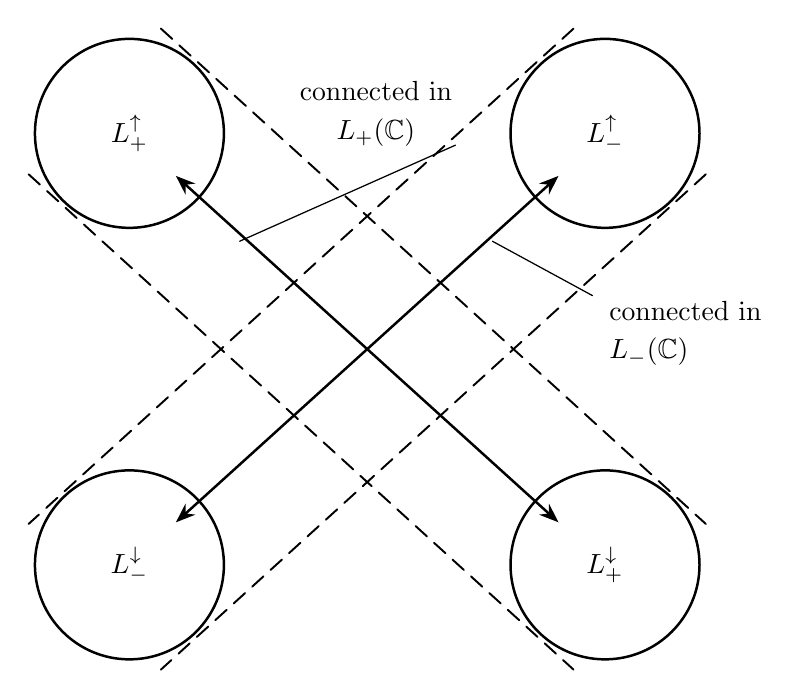
\begin{tikzpicture}[>=Stealth,line cap=round,line join=round,
    band/.style={dashed,dash pattern=on 5.5pt off 3.5pt,line width=.7pt},
    component/.style={fill=white,line width=.9pt},
    leader/.style={line width=.45pt}]
    % The dashed band flanking the L_+(C) connector.
    \draw[band] (-2.62, 4.07) -- ( 4.30,-2.22);
    \draw[band] (-4.30, 2.22) -- ( 2.62,-4.07);

    % The dashed band flanking the L_-(C) connector.
    \draw[band] ( 2.62, 4.07) -- (-4.30,-2.22);
    \draw[band] ( 4.30, 2.22) -- (-2.62,-4.07);

    % The four components of L.
    \draw[component] (-3.02, 2.74) circle (1.20);
    \draw[component] ( 3.02, 2.74) circle (1.20);
    \draw[component] (-3.02,-2.74) circle (1.20);
    \draw[component] ( 3.02,-2.74) circle (1.20);
    \node at (-3.02, 2.74) {$L^\uparrow_+$};
    \node at ( 3.02, 2.74) {$L^\uparrow_-$};
    \node at (-3.02,-2.74) {$L^\downarrow_-$};
    \node at ( 3.02,-2.74) {$L^\downarrow_+$};

    % The two connectors run into the components they join.
    \draw[<->,line width=.9pt] (-2.43, 2.20) -- ( 2.43,-2.20);
    \draw[<->,line width=.9pt] ( 2.43, 2.20) -- (-2.43,-2.20);

    % The two leader lines, each pointing at the connector it names.
    \node[align=center] at (0.11,2.99) {connected in\\[2pt]$L_+(\mathbb C)$};
    \draw[leader] (1.12,2.59) -- (-1.62,1.37);
    \node[anchor=west,align=left] at (2.95,0.20)
      {connected in\\[2pt]$L_-(\mathbb C)$};
    \draw[leader] (2.86,0.68) -- (1.59,1.37);
  \end{tikzpicture}
  \caption{Connectivity properties of the complex Lorentz group, $L(\mathbb C)$.
  There are two connected components: $L_+(\mathbb C)$, the proper complex
  Lorentz group, which contains $L^\uparrow_+$ and $L^\downarrow_+$; and
  $L_-(\mathbb C)$, which contains $L^\uparrow_-$ and $L^\downarrow_-$.}
  \label{fig:ch1-complex-lorentz-components}
\end{figure}
\endgroup
\clearpage
% PCT-SOURCE: pdf=038 print=026 kind=figure id=1-3
% Native reconstruction from the rendered source page.  The vertical hatch
% marks the two-particle continuum and the crossed hatch marks the
% three-particle continuum.
\begingroup
\renewcommand{\thefigure}{1-3}
\renewcommand{\figurename}{FIGURE}
\begin{figure}[t]
  \centering
  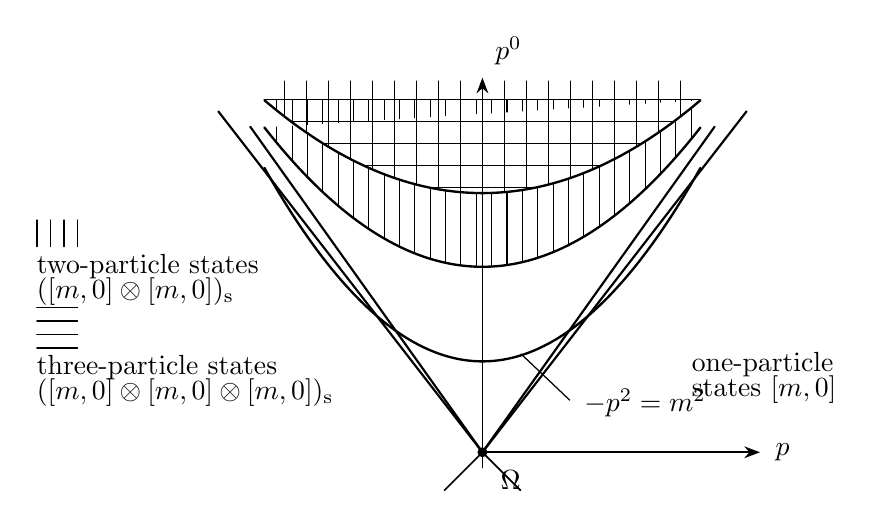
\begin{tikzpicture}[x=0.78cm,y=0.78cm,>=Stealth,
    line cap=round,line join=round]
    \begin{scope}[xshift=2.60cm]
    % The four straight spectral-cone rays.
    \draw[line width=.78pt] (-4.30,5.55) -- (0,0) -- (4.30,5.55);
    \draw[line width=.78pt] (-3.78,5.30) -- (0,0) -- (3.78,5.30);
    \draw[line width=.60pt] (-0.62,-0.62) -- (0,0) -- (0.62,-0.62);

    % Two-particle continuum: vertical hatching between the two-particle
    % threshold and the upper boundary.
    \begin{scope}
      \clip
        plot[domain=-3.55:3.55,samples=100]
          (\x,{3.02+0.18*\x*\x})
        -- (3.55,{4.22+0.12*3.55*3.55})
        plot[domain=3.55:-3.55,samples=100]
          (\x,{4.22+0.12*\x*\x}) -- cycle;
      \foreach \x in {-3.6,-3.35,...,3.6}
        \draw[line width=.38pt] (\x,2.85) -- (\x,5.95);
    \end{scope}

    % Three-particle continuum: crossed hatching above the upper boundary.
    \begin{scope}
      \clip
        plot[domain=-3.55:3.55,samples=100]
          (\x,{4.22+0.12*\x*\x})
        -- (3.55,6.05) -- (-3.55,6.05) -- cycle;
      \draw[step=.28cm,line width=.34pt] (-3.65,4.10) grid (3.65,6.10);
    \end{scope}

    % Curves bounding the mass shells and continua.
    \draw[line width=.85pt,domain=-3.55:3.55,samples=140]
      plot (\x,{1.48+0.25*\x*\x});
    \draw[line width=.85pt,domain=-3.55:3.55,samples=140]
      plot (\x,{3.02+0.18*\x*\x});
    \draw[line width=.85pt,domain=-3.55:3.55,samples=140]
      plot (\x,{4.22+0.12*\x*\x});

    % Axes, labels, and the vacuum point.
    \draw[->,line width=.60pt] (0,-0.25) -- (0,6.10)
      node[above right=1pt] {$p^0$};
    \draw[->,line width=.60pt] (0,0) -- (4.52,0)
      node[right=2pt] {$p$};
    \fill (0,0) circle (1.8pt);
    \node[below right=3pt] at (0,0) {$\Omega$};

    \draw[line width=.45pt] (0.63,1.60) -- (1.42,0.85);
    \node[right] at (1.50,0.80) {$-p^2=m^2$};

    \node[anchor=west] at (3.25,1.42) {one-particle};
    \node[anchor=west] at (3.25,1.02) {states $[m,0]$};
    \end{scope}

    % Legend for the two hatching patterns.
    \foreach \x in {-3.92,-3.70,-3.48,-3.26}
      \draw[line width=.55pt] (\x,3.35) -- (\x,3.78);
    \node[anchor=west] at (-4.08,3.02) {two-particle states};
    \node[anchor=west] at (-4.08,2.62)
      {$([m,0]\otimes[m,0])_{\mathrm{s}}$};
    \foreach \y in {1.70,1.92,2.14,2.36}
      \draw[line width=.55pt] (-3.92,\y) -- (-3.26,\y);
    \node[anchor=west] at (-4.08,1.38) {three-particle states};
    \node[anchor=west] at (-4.08,0.98)
      {$([m,0]\otimes[m,0]\otimes[m,0])_{\mathrm{s}}$};
  \end{tikzpicture}
  \caption{The spectrum of a theory of neutral scalar mesons of mass $m$
  without bound states.}
  \label{fig:1-3}
\end{figure}
\endgroup
\clearpage
% PCT-SOURCE: pdf=070 print=58 kind=figure id=2-1
% Native reconstruction from the rendered source page.  The contour runs
% along three horizontal lines; the arrowheads carry their orientation.
\begingroup
\renewcommand{\thefigure}{2-1}
\renewcommand{\figurename}{FIGURE}
\begin{figure}[t]
  \centering
  \begin{tikzpicture}[>=Stealth,line cap=round,line join=round,
    contour/.style={line width=.75pt}]
    % The imaginary axis of the z plane.
    \draw[->,line width=.7pt] (0,-3.03) -- (0,3.28);
    \node at (1.94,3.15) {$z$};

    % The upper line, traversed to the right.
    \draw[contour,->] (-4.06,1.65) -- (3.94,1.65);

    % The middle line, traversed to the left.
    \draw[contour,->] (4.14,0) -- (-1.11,0);
    \draw[contour] (-1.11,0) -- (-4.06,0);

    % The lower line, traversed to the right.
    \draw[contour,->] (-4.06,-1.60) -- (0.86,-1.60);
    \draw[contour] (0.86,-1.60) -- (4.14,-1.60);

    \node at ( 0.33, 0.31) {$a$};
    \node at (-0.29,-1.92) {$b$};
  \end{tikzpicture}
  \caption{The contour $C$ in the plane of $z=\xi-i\eta$.}
  \label{fig:2-1}
  \label{fig:ch2-contour}
\end{figure}
\endgroup
\clearpage
% PCT-SOURCE: pdf=077 print=65 kind=figure id=2-2
% Native reconstruction of the single-valuedness diagram.  The projected
% geometry follows the printed drawing, with the tube boundary at left, the
% two endpoint configurations, and the common Lorentz-transformed endpoint.
\begingroup
\renewcommand{\thefigure}{2-2}
\renewcommand{\figurename}{FIGURE}
\begin{figure}[htbp]
  \centering
  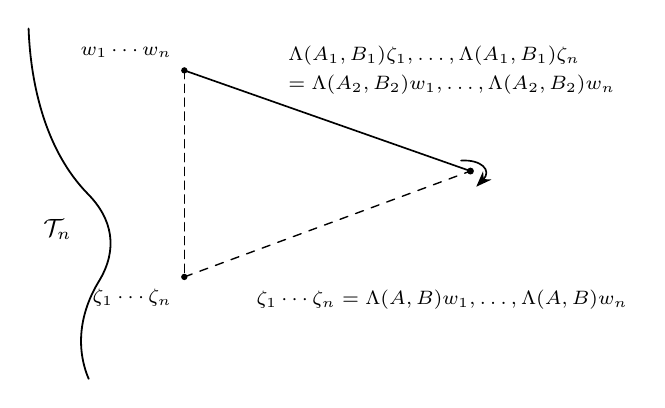
\begin{tikzpicture}[x=0.92cm,y=0.83cm,>=Stealth,line cap=round,
    line join=round]
    % A projected boundary of the extended tube.
    \draw[line width=.65pt]
      (-2.15,2.72)
        .. controls (-2.12,1.82) and (-1.90,.84) .. (-1.34,.20)
        .. controls (-.98,-.20) and (-.92,-.66) .. (-1.17,-1.13)
        .. controls (-1.45,-1.63) and (-1.50,-2.17) .. (-1.32,-2.64);
    \node[font=\small] at (-1.75,-.36) {$\mathcal{T}_n$};

    % The two configurations joined by the vertical path in the tube.
    \fill (0.00,2.08) circle (1.15pt);
    \fill (0.00,-1.08) circle (1.15pt);
    \draw[densely dashed,line width=.5pt] (0,2.08) -- (0,-1.08);
    \node[above left=1pt,font=\scriptsize] at (0,2.08) {$w_1\cdots w_n$};
    \node[below left=1pt,font=\scriptsize] at (0,-1.08)
      {$\zeta_1\cdots\zeta_n$};

    % The two endpoint paths meet at the transformed configuration.
    \coordinate (q) at (3.95,.54);
    \fill (q) circle (1.25pt);
    \draw[line width=.6pt] (0,2.08) -- (q);
    \draw[dashed,line width=.5pt] (0,-1.08) -- (q);
    \draw[->,line width=.6pt] (3.82,.70) .. controls (4.10,.72) and
      (4.25,.55) .. (4.03,.30);
    \node[align=left,font=\scriptsize,anchor=west] at (1.30,2.30)
      {$\Lambda(A_1,B_1)\zeta_1,\ldots,\Lambda(A_1,B_1)\zeta_n$};
    \node[align=left,font=\scriptsize,anchor=west] at (1.30,1.86)
      {$=\Lambda(A_2,B_2)w_1,\ldots,\Lambda(A_2,B_2)w_n$};

    % Lower endpoint notation in the source drawing.
    \node[align=left,font=\scriptsize,anchor=west] at (.86,-1.43)
      {$\zeta_1\cdots\zeta_n=\Lambda(A,B)w_1,\ldots,\Lambda(A,B)w_n$};
  \end{tikzpicture}
  \caption{The single-valuedness of the functions as defined throughout the
  extended tube $\mathcal{T}'_{n}$ follows from the fact that, if
  $w_1,\ldots,w_n$ and $\Lambda w_1,\ldots,\Lambda w_n\in\mathcal{T}_{n}$,
  then there is a curve of proper complex Lorentz transformations
  $\{\Lambda(t);\ 0\leq t\leq1\}$ with $\Lambda(0)=\mathbf{1}$,
  $\Lambda(1)=\Lambda$, such that
  $\Lambda(t)w_1,\ldots,\Lambda(t)w_n\in\mathcal{T}_{n}$ for
  $0\leq t\leq1$.  Here $A=A_1^{-1}A_2$, $B=B_1^{-1}B_2$.}
  \label{fig:2-2}
\end{figure}
\endgroup
\clearpage
% PCT-SOURCE: pdf=084 print=72 kind=figure id=2-3
% Native reconstruction from the rendered source page.  The double cone, the
% two oblique separating planes, and the three space-like vectors all share
% the apex, as in the printed drawing.
\begingroup
\renewcommand{\thefigure}{2-3}
\renewcommand{\figurename}{FIGURE}
\begin{figure}[htbp]
  \centering
  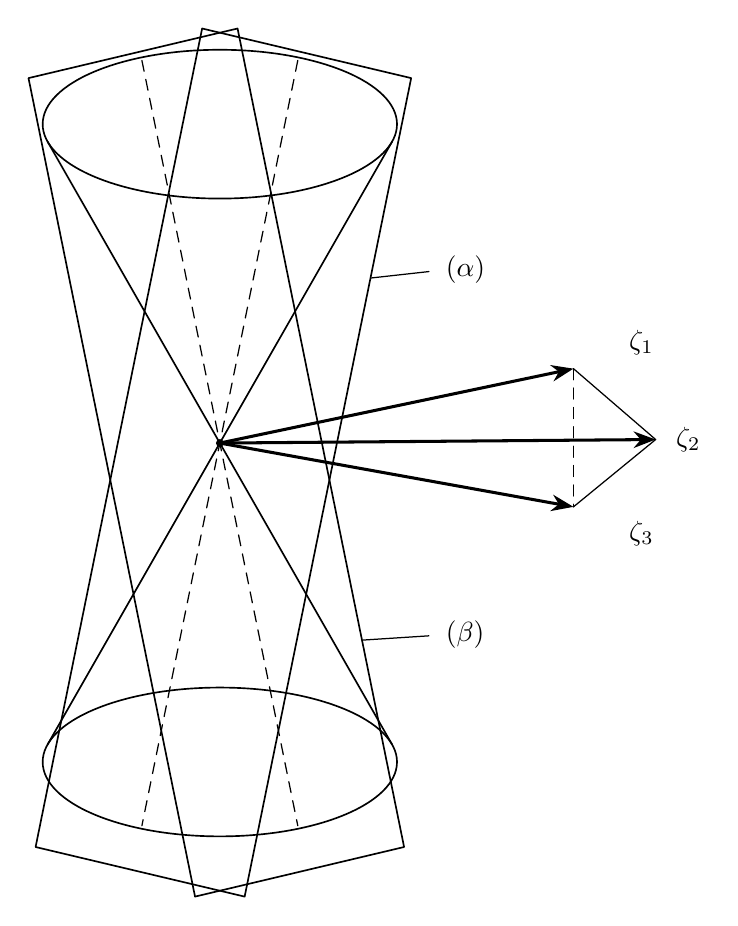
\begin{tikzpicture}[x=0.90cm,y=0.90cm,>=Stealth,line cap=round,
    line join=round,
    edge/.style={line width=.6pt},
    hidden/.style={dashed,dash pattern=on 4pt off 3pt,line width=.45pt}]
    % The plus and minus light cones with their rims.
    \draw[edge] (-2.431, 4.254) -- (0,0) -- (2.431, 4.254);
    \draw[edge] (-2.431,-4.254) -- (0,0) -- (2.431,-4.254);
    \draw[edge] (0, 4.50) ellipse (2.50 and 1.05);
    \draw[edge] (0,-4.50) ellipse (2.50 and 1.05);

    % Plane (alpha): its long edges lean to the left going down.
    \draw[edge] (2.70,5.15) -- (-0.25,5.85) -- (-2.60,-5.70)
      -- (0.35,-6.40) -- cycle;
    \draw[hidden] (1.10,5.40) -- (-1.10,-5.40);

    % Plane (beta): the opposite oblique orientation.
    \draw[edge] (-2.70,5.15) -- (0.25,5.85) -- (2.60,-5.70)
      -- (-0.35,-6.40) -- cycle;
    \draw[hidden] (-1.10,5.40) -- (1.10,-5.40);

    \draw[line width=.45pt] (2.95, 2.42) -- (2.14, 2.33);
    \node[anchor=west] at (3.05, 2.45) {$(\alpha)$};
    \draw[line width=.45pt] (2.95,-2.72) -- (2.02,-2.78);
    \node[anchor=west] at (3.05,-2.70) {$(\beta)$};

    % The three space-like vectors of the Jost point.
    \draw[->,line width=1.1pt] (0,0) -- (4.99, 1.05);
    \draw[->,line width=1.1pt] (0,0) -- (6.15, 0.05);
    \draw[->,line width=1.1pt] (0,0) -- (4.99,-0.90);
    \fill (0,0) circle (1.4pt);
    \draw[line width=.45pt] (4.99, 1.05) -- (6.15,0.05);
    \draw[line width=.45pt] (4.99,-0.90) -- (6.15,0.05);
    \draw[hidden] (4.99,1.05) -- (4.99,-0.90);
    \node at (5.95, 1.42) {$\zeta_1$};
    \node[anchor=west] at (6.30, 0.05) {$\zeta_2$};
    \node at (5.95,-1.28) {$\zeta_3$};
  \end{tikzpicture}
  \caption{The cone of space-like vectors corresponding to a Jost point
  $\zeta_1,\zeta_2,\zeta_3$.  The planes $(\alpha)$ and $(\beta)$ separate
  the cone spanned by $\zeta_1,\zeta_2,\zeta_3$ from the interior of the plus
  and minus light cones.}
  \label{fig:2-3}
\end{figure}
\endgroup
\clearpage
% PCT-SOURCE: pdf=085 print=73 kind=figure id=2-4
% Projected native reconstruction of the two configurations in the source.
\begingroup
\renewcommand{\thefigure}{2.4}
\renewcommand{\figurename}{FIGURE}
\begin{figure}[htbp]
  \centering
  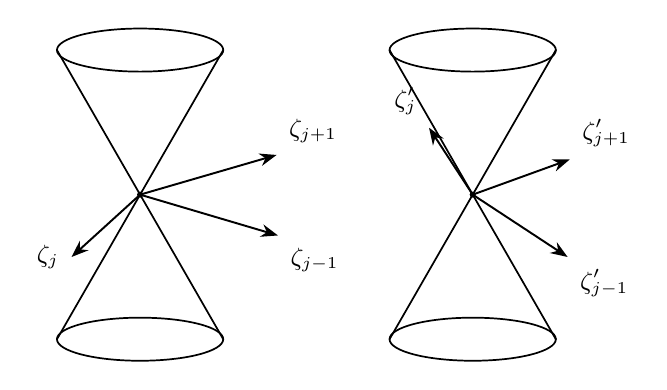
\begin{tikzpicture}[x=0.88cm,y=0.72cm,>=Stealth,line cap=round,
    line join=round]
    % Left cone.
    \coordinate (L) at (-2.55,0);
    \draw[line width=.62pt] (-3.75,2.55) arc (180:360:1.20 and .38);
    \draw[line width=.62pt] (-3.75,2.55) -- (L) -- (-1.35,2.55);
    \draw[line width=.62pt] (-3.75,2.55) arc (180:0:1.20 and .38);
    \draw[line width=.62pt] (-3.75,-2.55) arc (180:360:1.20 and .38);
    \draw[line width=.62pt] (-3.75,-2.55) -- (L) -- (-1.35,-2.55);
    \draw[line width=.62pt] (-3.75,-2.55) arc (180:0:1.20 and .38);
    \fill (L) circle (1.1pt);
    \draw[->,line width=.7pt] (L) -- (-.58,.70);
    \draw[->,line width=.7pt] (L) -- (-.56,-.72);
    \draw[->,line width=.7pt] (L) -- (-3.54,-1.10);
    \node[above right=1pt,font=\small] at (-.58,.70) {$\zeta_{j+1}$};
    \node[below right=1pt,font=\small] at (-.56,-.72) {$\zeta_{j-1}$};
    \node[left=1pt,font=\small] at (-3.54,-1.10) {$\zeta_j$};

    % Right cone, with primed vectors.
    \coordinate (R) at (2.25,0);
    \draw[line width=.62pt] (1.05,2.55) arc (180:360:1.20 and .38);
    \draw[line width=.62pt] (1.05,2.55) -- (R) -- (3.45,2.55);
    \draw[line width=.62pt] (1.05,2.55) arc (180:0:1.20 and .38);
    \draw[line width=.62pt] (1.05,-2.55) arc (180:360:1.20 and .38);
    \draw[line width=.62pt] (1.05,-2.55) -- (R) -- (3.45,-2.55);
    \draw[line width=.62pt] (1.05,-2.55) arc (180:0:1.20 and .38);
    \fill (R) circle (1.1pt);
    \draw[->,line width=.7pt] (R) -- (1.62,1.18);
    \draw[->,line width=.7pt] (R) -- (3.65,.62);
    \draw[->,line width=.7pt] (R) -- (3.62,-1.10);
    \node[above left=1pt,font=\small] at (1.62,1.18) {$\zeta'_j$};
    \node[above right=1pt,font=\small] at (3.65,.62) {$\zeta'_{j+1}$};
    \node[below right=1pt,font=\small] at (3.62,-1.10) {$\zeta'_{j-1}$};
  \end{tikzpicture}
  \caption{A configuration of vectors $\zeta_{j-1},\zeta_j,\zeta_{j+1}$
  appearing for a Jost point of $\mathcal{T}'_{n}$ and
  $P(j,j+1)\mathcal{T}'_{n}$.  The $\zeta'$'s are obtained from the $\zeta$'s
  by $\zeta'_{j-1}=\zeta_{j-1}+\zeta_j$, $\zeta'_j=-\zeta_j$,
  $\zeta'_{j+1}=\zeta_{j+1}+\zeta_j$.}
  \label{fig:2-4}
\end{figure}
\endgroup
\clearpage
% PCT-SOURCE: pdf=086 print=74 kind=figure id=2-5
% Native reconstruction of the two domains meeting the interval [a,b].
\begingroup
\renewcommand{\thefigure}{2-5}
\renewcommand{\figurename}{FIGURE}
\begin{figure}[htbp]
  \centering
  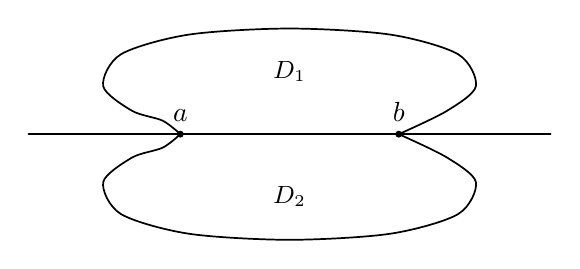
\begin{tikzpicture}[x=1.02cm,y=.78cm,line cap=round,line join=round]
    \draw[line width=.62pt] (-3.25,0) -- (3.25,0);
    \fill (-1.36,0) circle (1.25pt);
    \fill (1.36,0) circle (1.25pt);
    \node[above=1pt] at (-1.36,0) {$a$};
    \node[above=1pt] at (1.36,0) {$b$};
    \draw[line width=.62pt]
      plot[smooth] coordinates {
        (-1.36,0) (-1.58,.22) (-1.96,.38) (-2.32,.78)
        (-2.10,1.30) (-1.26,1.62) (0,1.72) (1.26,1.62)
        (2.10,1.30) (2.32,.78) (1.96,.38) (1.36,0)};
    \draw[line width=.62pt]
      plot[smooth] coordinates {
        (-1.36,0) (-1.58,-.22) (-1.96,-.38) (-2.32,-.78)
        (-2.10,-1.30) (-1.26,-1.62) (0,-1.72) (1.26,-1.62)
        (2.10,-1.30) (2.32,-.78) (1.96,-.38) (1.36,0)};
    \node[font=\small] at (0,1.02) {$D_1$};
    \node[font=\small] at (0,-1.02) {$D_2$};
  \end{tikzpicture}
  \caption{Domains $D_1$ and $D_2$, of definition of $F_1$ and $F_2$,
  respectively.}
  \label{fig:2-5}
  \label{fig:ch2-edge-wedge-domains}
\end{figure}
\endgroup
\clearpage
\begingroup
\renewcommand{\thefigure}{2-6}
\renewcommand{\figurename}{FIGURE}
\begin{figure}[t]
  \centering
  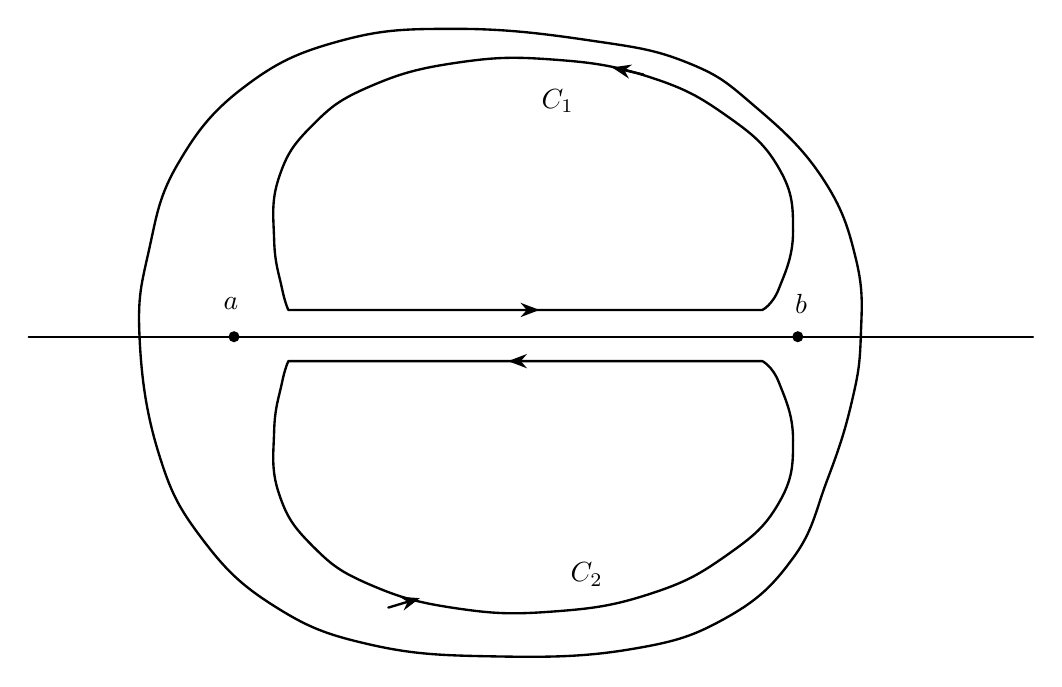
\begin{tikzpicture}[>=Stealth,line cap=round,line join=round,
    curve/.style={line width=.85pt},
    orient/.style={->,line width=.85pt}]
    % The real axis.
    \draw[line width=.6pt] (-6.19,0) -- (6.57,0);

    % The boundary of the union of the two domains.
    \draw[curve] plot[smooth cycle,tension=.72] coordinates {
      (-4.78, 0.00) (-4.66, 1.10) (-4.29, 2.20) (-3.44, 3.18) (-2.22, 3.76)
      (-0.75, 3.91) ( 0.96, 3.76) ( 2.18, 3.48) ( 3.03, 2.93) ( 3.89, 2.02)
      ( 4.32, 0.98) ( 4.38, 0.00) ( 4.26,-0.85) ( 3.95,-1.83) ( 3.52,-2.81)
      ( 2.67,-3.57) ( 1.45,-3.97) (-0.26,-4.06) (-1.85,-3.91) (-3.07,-3.42)
      (-3.99,-2.56) (-4.54,-1.47)};

    % C_1, in D_1.
    \draw[curve] plot[smooth,tension=.75] coordinates {
      ( 3.13, 0.34) ( 3.34, 0.61) ( 3.52, 1.34) ( 3.34, 2.14) ( 2.67, 2.81)
      ( 1.69, 3.30) ( 0.47, 3.52) (-0.75, 3.48) (-1.85, 3.18) (-2.58, 2.69)
      (-3.01, 2.02) (-3.07, 1.22) (-2.97, 0.61) (-2.89, 0.34)} -- cycle;
    \draw[orient] (-0.10,0.34) -- (0.30,0.34);
    \draw[orient] ( 1.62,3.33) -- (1.22,3.42);
    \node at (0.53,2.99) {$C_1$};

    % C_2, in D_2.
    \draw[curve] plot[smooth,tension=.75] coordinates {
      ( 3.13,-0.31) ( 3.34,-0.58) ( 3.52,-1.31) ( 3.34,-2.11) ( 2.67,-2.78)
      ( 1.69,-3.27) ( 0.47,-3.49) (-0.75,-3.45) (-1.85,-3.15) (-2.58,-2.66)
      (-3.01,-1.99) (-3.07,-1.19) (-2.97,-0.58) (-2.89,-0.31)} -- cycle;
    \draw[orient] ( 0.30,-0.31) -- (-0.10,-0.31);
    \draw[orient] (-1.62,-3.44) -- (-1.22,-3.32);
    \node at (0.90,-3.02) {$C_2$};

    % The interval a<x<b.
    \fill (-3.58,0) circle (2.0pt);
    \fill ( 3.58,0) circle (2.0pt);
    \node at (-3.62,0.42) {$a$};
    \node at ( 3.62,0.42) {$b$};
  \end{tikzpicture}
  \caption{The contours $C_1$ and $C_2$.}
  \label{fig:2-6}
  \label{fig:ch2-edge-wedge-contours}
\end{figure}
\endgroup
\clearpage
\begingroup
\renewcommand{\thefigure}{2-7}
\renewcommand{\figurename}{FIGURE}
\begin{figure}[htbp]
  \centering
  \begin{tikzpicture}[x=0.95cm,y=0.95cm,>=Stealth,line cap=round,
    line join=round,axis@/.style={line width=.7pt}]
    % The z plane.
    \draw[axis@,->] (0,-3.97) -- (0,6.69);
    \draw[axis@] (-3.05,0) -- (2.15,0);
    \draw[line width=.85pt] (0,0) circle (2.08);
    \node at (-1.68,4.70) {$z$-plane};
    \node[anchor=east] at (-2.15,-0.42) {$z=-1$};
    \node[anchor=west] at ( 2.22,-0.42) {$z=1$};

    % The w plane.
    \begin{scope}[shift={(7.69,0)}]
      \draw[axis@,->] (0,-3.97) -- (0,6.51);
      \draw[axis@] (-3.38,0) -- (3.57,0);
      \draw[line width=.85pt] (0,2.17) circle (3.05);
      \fill (0,2.17) circle (1.5pt);
      \node at (3.12,5.50) {$w$-plane};
      \node[anchor=east] at (-2.05,-0.42) {$w=-1$};
      \node[anchor=west] at ( 2.28,-0.42) {$w=1$};

      % The center of the image circle, named above the drawing.
      \draw[line width=.5pt] (-3.10,7.05) -- (-0.06,2.22);
      \node[anchor=west,font=\small] at (-3.45,7.52)
        {$\displaystyle
          w=\frac{4\bigl[u(1+|u|^2)-(1+u^2)\operatorname{Re}u\bigr]}
                 {\bigl[(1+|u|^2)(1+u^2)-4u\operatorname{Re}u\bigr]}$};
    \end{scope}
  \end{tikzpicture}
  \caption{Illustration of the mapping $w=(u+z)/(1+uz)$.  As $z$ runs over
  the unit circle $|z|=1$, $w$ runs over the circle indicated.  The points
  $z=\pm1$ always are mapped into $w=\pm1$.}
  \label{fig:2-7}
  \label{fig:ch2-mobius-map}
\end{figure}
\endgroup
\clearpage
\begingroup
\renewcommand{\thefigure}{A.1}
\renewcommand{\figurename}{Figure}
\begin{figure}[htbp]
  \centering
  \begin{tikzpicture}[>=Stealth,line cap=round,line join=round]
    % The causal diamond and its horizontal diagonal.
    \draw[line width=.85pt]
      (-3.15,0) -- (0,3.15) -- (3.15,0) -- (0,-3.15) -- cycle;
    \draw[line width=.85pt] (-3.15,0) -- (3.15,0);

    % The space and time axes, both set off from the diamond as in the source.
    \draw[->,line width=.7pt] (3.67,0) -- (5.67,0) node[right=2pt] {$x$};
    \draw[->,line width=.7pt] (3.15,1.20) -- (3.15,2.66);
    \node[anchor=west] at (3.30,1.90) {$t$};

    % The interval on which g=1.
    \draw[line width=.55pt] (-3.15,-0.14) -- (-3.15,-1.10);
    \draw[line width=.55pt] ( 3.15,-0.14) -- ( 3.15,-1.10);
    \draw[<->,line width=.6pt] (-3.09,-0.76) -- (3.09,-0.76);
    \node[fill=white,inner sep=1.5pt] at (0,-0.76) {$g=1$};
  \end{tikzpicture}
  \caption{The dependence domain of the region where $g=1$.}
  \label{fig:A-1}
\end{figure}
\endgroup
\clearpage
% PCT-SOURCE: pdf=200 print=188 kind=figure id=A.2
% Native reconstruction of the Ising phase diagram on source page 188.
\begingroup
\renewcommand{\thefigure}{A.2}
\renewcommand{\figurename}{Figure}
\begin{figure}[htbp]
  \centering
  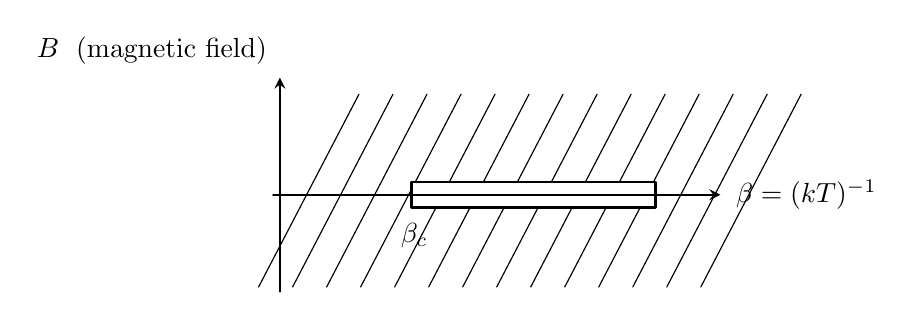
\begin{tikzpicture}[x=1.08cm,y=.96cm,>=stealth,line cap=round,
    line join=round]
    % Diagonal hatching marks the two-phase line's surrounding phase
    % diagram.  The white strip is the B=0 part for beta >= beta_c.
    \foreach \x in {-.25,.15,.55,.95,1.35,1.75,2.15,2.55,2.95,3.35,3.75,4.15,4.55,4.95}
      \draw[line width=.42pt] (\x,-1.22) -- ++(1.18,2.55);

    \draw[->,line width=.75pt] (0,-1.28) -- (0,1.55)
      node[above left=1pt] {$B$\; (magnetic field)};
    \draw[->,line width=.75pt] (-.08,0) -- (5.18,0)
      node[right=2pt] {$\beta=(kT)^{-1}$};

    % The critical half-line lies on B=0.  Its outlined strip preserves the
    % double ruled line visible in the scan.
    \fill[white] (1.55,-.17) rectangle (4.42,.17);
    \draw[line width=.9pt] (1.55,-.17) rectangle (4.42,.17);
    \draw[line width=.55pt] (1.55,0) -- (4.42,0);
    \node[below=2pt] at (1.58,-.17) {$\beta_c$};
  \end{tikzpicture}
  \caption{Phase diagram of the Ising ferromagnet (nearest-neighbor interaction). The phase is unique and the correlation functions decay exponentially for all values of $\beta$ and $B$ except those satisfying $B=0$, $\beta_c\leq\beta<\infty$, where there are exactly two phases. The phase diagram for the $\lambda\varphi^4+\mu\varphi^2+\nu\varphi$ model is similar, with $B$ replaced by $\nu$ and $\beta$ by $\lambda$. The solution is known to be unique for $\nu\ne0$ and for all sufficiently small positive $\lambda$. It is known that at least two solutions, I and II, exist for all sufficiently large $\lambda$ with $\varphi\to-\varphi$ symmetry broken in the sense that $\matrixel{\Omega_{0I}}{\varphi_1(x)}{\Omega_{0I}}=-\matrixel{\Omega_{0II}}{\varphi_1(x)}{\Omega_{0II}}\ne0$.}
  \label{fig:A-2}
\end{figure}
\endgroup
\clearpage
% PCT-SOURCE: pdf=210 print=198 kind=figure id=A.3
% Native reconstruction of the state profiles and automorphism arrows on
% source page 198.  The curves are schematic profiles, as in the source.
\begingroup
\renewcommand{\thefigure}{A.3}
\renewcommand{\figurename}{Figure}
\begin{figure}[p]
  \centering
\resizebox{\textwidth}{!}{%
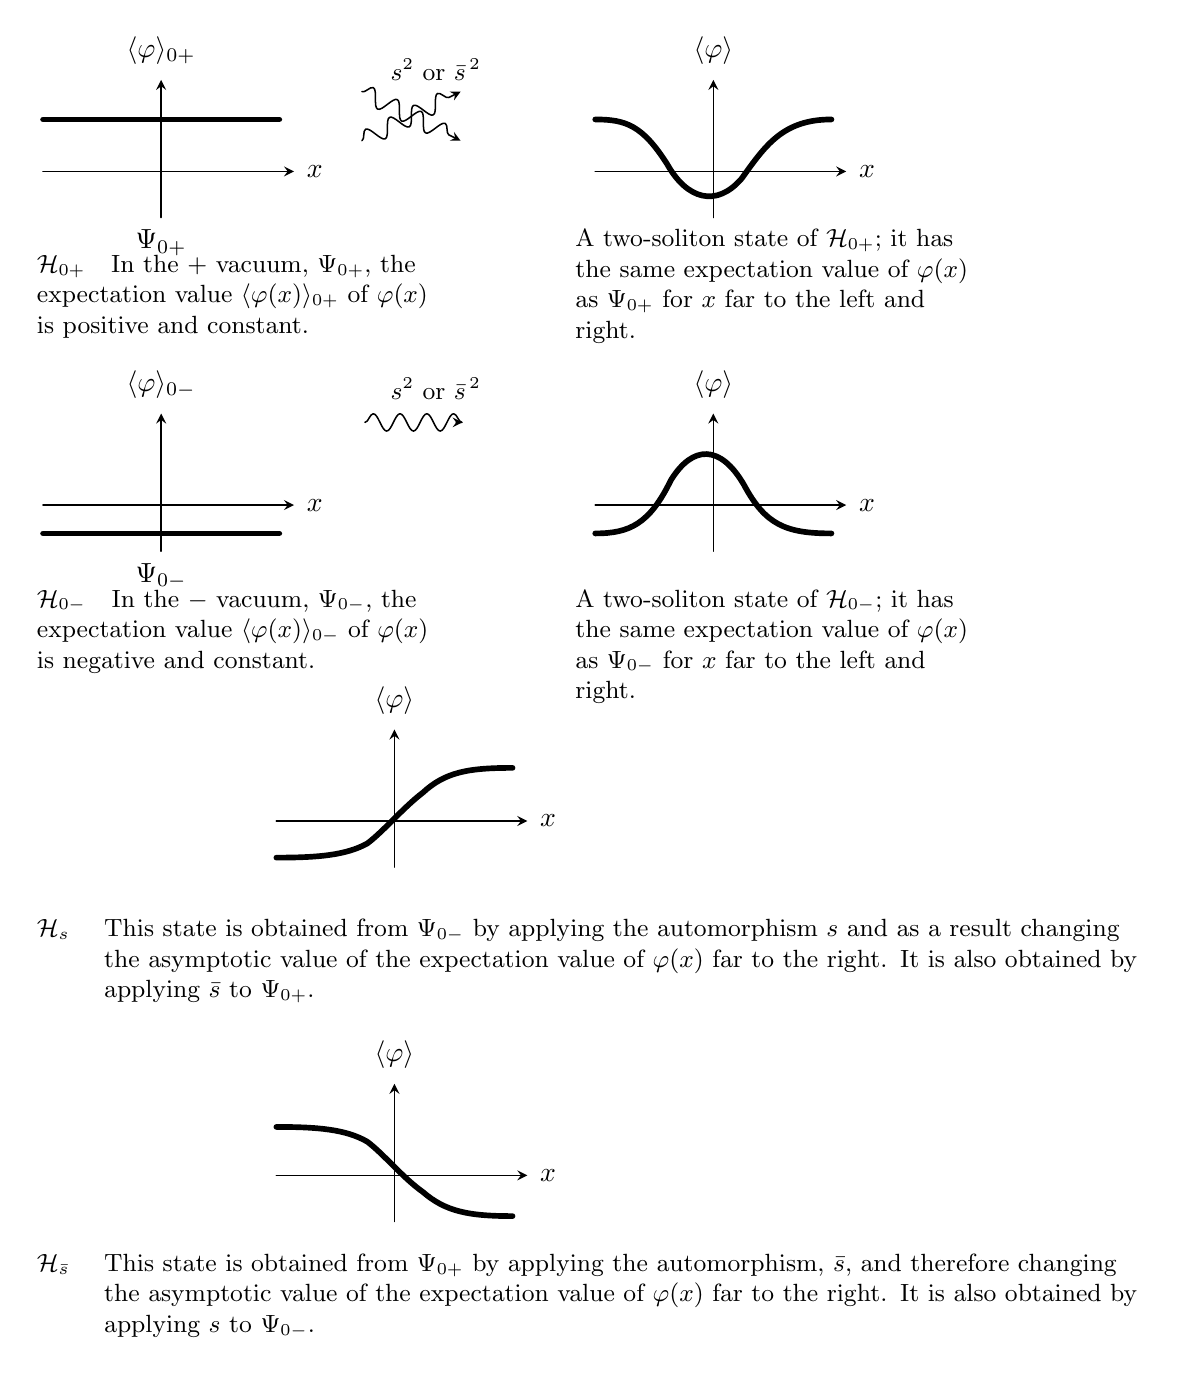
\begin{tikzpicture}[x=.75cm,y=.75cm,>=stealth,line cap=round,
    line join=round]
    % Reusable axes for the four small profiles.
    \newcommand{\pctaxes}[1]{%
      \draw[->,line width=.6pt] (#1-2.0,0) -- (#1+2.25,0)
        node[right=1pt] {$x$};%
      \draw[->,line width=.6pt] (#1, -.78) -- (#1,1.55);%
    }

    % Top-left: the positive vacuum.
    \begin{scope}[shift={(2.35,13.2)}]
      \pctaxes{0}
      \draw[line width=2.05pt] (-2.0,.88) -- (2.0,.88);
      \node[above=2pt] at (0,1.55) {$\langle\varphi\rangle_{0+}$};
      \node[below=1pt] at (0,-.78) {$\Psi_{0+}$};
    \end{scope}
    \node[anchor=north west,text width=5.2cm,align=left,font=\small]
      at (.08,11.95) {$\mathcal H_{0+}$\quad In the $+$ vacuum, $\Psi_{0+}$, the expectation value $\langle\varphi(x)\rangle_{0+}$ of $\varphi(x)$ is positive and constant.};

    % Top-right: a two-soliton profile in the positive sector.
    \begin{scope}[shift={(11.7,13.2)}]
      \pctaxes{0}
      \draw[line width=2.05pt]
        (-2.0,.88) .. controls (-1.48,.88) and (-1.20,.78) .. (-.78,.12)
        .. controls (-.45,-.47) and (.05,-.62) .. (.48,-.12)
        .. controls (.88,.44) and (1.18,.88) .. (2.0,.88);
      \node[above=2pt] at (0,1.55) {$\langle\varphi\rangle$};
    \end{scope}
    \node[anchor=north west,text width=5.15cm,align=left,font=\small]
      at (9.2,12.38) {A two-soliton state of $\mathcal H_{0+}$; it has the same expectation value of $\varphi(x)$ as $\Psi_{0+}$ for $x$ far to the left and right.};

    % The crossed wavy arrows between the first row of panels.
    \node[font=\small] at (7.0,14.92) {$s^2$ or $\bar s^{\,2}$};
    \draw[->,line width=.55pt,decorate,
      decoration={snake,amplitude=.11cm,segment length=.34cm}]
      (5.75,14.55) -- (7.42,13.72);
    \draw[->,line width=.55pt,decorate,
      decoration={snake,amplitude=.11cm,segment length=.34cm}]
      (5.75,13.72) -- (7.42,14.55);

    % Middle-left: the negative vacuum.
    \begin{scope}[shift={(2.35,7.55)}]
      \pctaxes{0}
      \draw[line width=2.05pt] (-2.0,-.48) -- (2.0,-.48);
      \node[above=2pt] at (0,1.55) {$\langle\varphi\rangle_{0-}$};
      \node[below=1pt] at (0,-.78) {$\Psi_{0-}$};
    \end{scope}
    \node[anchor=north west,text width=5.2cm,align=left,font=\small]
      at (.08,6.28) {$\mathcal H_{0-}$\quad In the $-$ vacuum, $\Psi_{0-}$, the expectation value $\langle\varphi(x)\rangle_{0-}$ of $\varphi(x)$ is negative and constant.};

    % Middle-right: a two-soliton profile in the negative sector.
    \begin{scope}[shift={(11.7,7.55)}]
      \pctaxes{0}
      \draw[line width=2.05pt]
        (-2.0,-.48) .. controls (-1.42,-.48) and (-1.08,-.32) .. (-.72,.42)
        .. controls (-.35,1.02) and (.12,1.03) .. (.52,.34)
        .. controls (.88,-.33) and (1.22,-.48) .. (2.0,-.48);
      \node[above=2pt] at (0,1.55) {$\langle\varphi\rangle$};
    \end{scope}
    \node[anchor=north west,text width=5.15cm,align=left,font=\small]
      at (9.2,6.28) {A two-soliton state of $\mathcal H_{0-}$; it has the same expectation value of $\varphi(x)$ as $\Psi_{0-}$ for $x$ far to the left and right.};

    % The single wavy arrow in the second row.
    \node[font=\small] at (7.0,9.52) {$s^2$ or $\bar s^{\,2}$};
    \draw[->,line width=.55pt,decorate,
      decoration={snake,amplitude=.11cm,segment length=.34cm}]
      (5.8,8.95) -- (7.45,8.95);

    % Profile obtained by applying s to the positive vacuum.
    \begin{scope}[shift={(6.3,2.2)}]
      \pctaxes{0}
      \draw[line width=2.05pt]
        (-2.0,-.62) .. controls (-1.3,-.62) and (-.82,-.58) .. (-.46,-.38)
        .. controls (-.18,-.17) and (.14,.22) .. (.48,.48)
        .. controls (.86,.83) and (1.25,.9) .. (2.0,.9);
      \node[above=2pt] at (0,1.55) {$\langle\varphi\rangle$};
    \end{scope}
    \node[anchor=north west,text width=1.0cm,align=left,font=\small]
      at (.08,.7) {$\mathcal H_s$};
    \node[anchor=north west,text width=13.2cm,align=left,font=\small]
      at (1.22,.7) {This state is obtained from $\Psi_{0-}$ by applying the automorphism $s$ and as a result changing the asymptotic value of the expectation value of $\varphi(x)$ far to the right. It is also obtained by applying $\bar s$ to $\Psi_{0+}$.};

    % Profile obtained by applying s to the negative vacuum.
    \begin{scope}[shift={(6.3,-3.8)}]
      \pctaxes{0}
      \draw[line width=2.05pt]
        (-2.0,.82) .. controls (-1.3,.82) and (-.82,.78) .. (-.46,.57)
        .. controls (-.18,.36) and (.14,-.04) .. (.48,-.28)
        .. controls (.86,-.61) and (1.25,-.69) .. (2.0,-.69);
      \node[above=2pt] at (0,1.55) {$\langle\varphi\rangle$};
    \end{scope}
    \node[anchor=north west,text width=1.0cm,align=left,font=\small]
      at (.08,-4.97) {$\mathcal H_{\bar s}$};
    \node[anchor=north west,text width=13.2cm,align=left,font=\small]
      at (1.22,-4.97) {This state is obtained from $\Psi_{0+}$ by applying the automorphism, $\bar s$, and therefore changing the asymptotic value of the expectation value of $\varphi(x)$ far to the right. It is also obtained by applying $s$ to $\Psi_{0-}$.};
  \end{tikzpicture}%
}
  \caption{\sloppy Behavior of $\langle\varphi(x)\rangle$ as a function of space coordinate for some typical states of $\mathcal{P}(\varphi^4)_2$ in the two-phase region. The action of the automorphisms $s^2=s\circ s$, $\bar{s}^{\,2}=\bar{s}\circ\bar{s}$ and $s\circ\bar{s}$ are indicated by the wavy arrows. In particular, note that the action of the composite automorphism $s\circ\bar{s}$ is to change the asymptotic value of the expectation value of $\varphi(x)$ both to the right and left.}
  \label{fig:A-3}
\end{figure}
\endgroup
\clearpage
\end{document}
